\section{aTag Enhancements}
We have demonstrated a tag format consisting of an attribute superset identifier and an bitmask, which can be used for easily decoding attributes associated with a flow. We will now present some improvements to this format.

%\subsection{Encoding Non-Binary Attributes}


\subsection{Variable Length Identifiers}
It is unlikely that all attribute supersets will be the same width, causing different tags to use a different number of bits. If we are using a fixed-width field in the packet headers for the tags, then it must be at least the size of the largest tag, and all smaller tags must be padded to the size of the largest tag. This wastes space which could perhaps be used in a more clever fashion.

\begin{figure}[t!] 
\begin{minipage}{1\linewidth}
\begin{subfigure}[c]{0.96\linewidth}
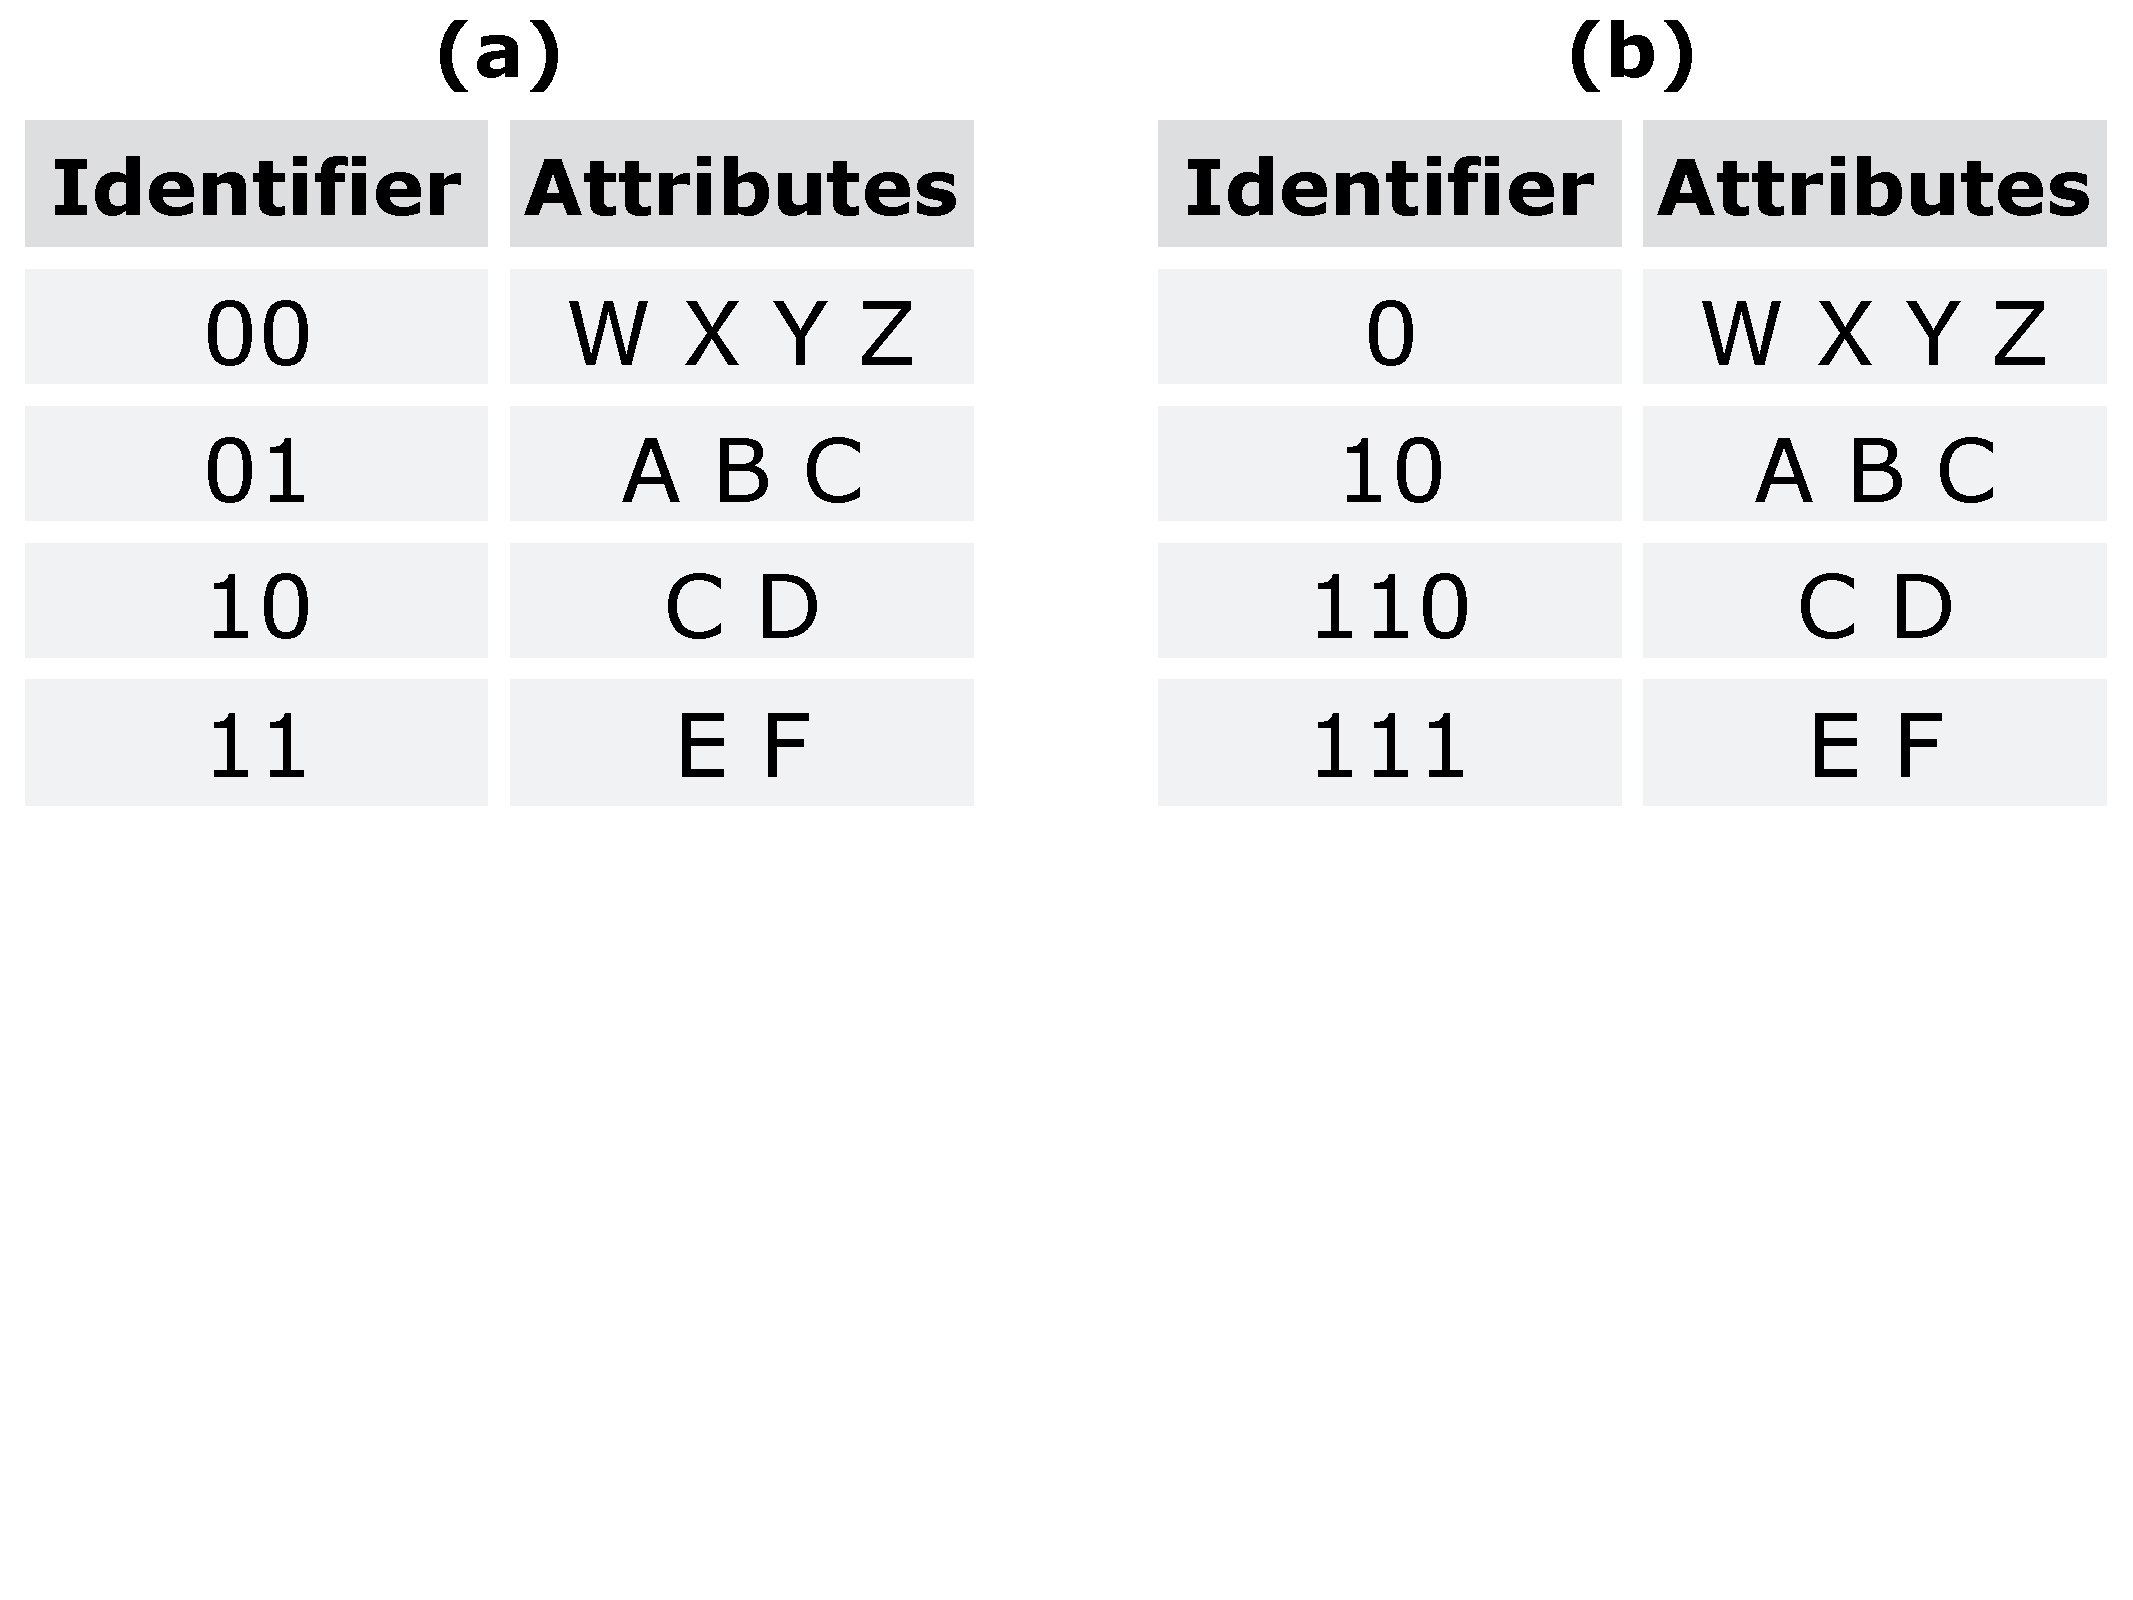
\includegraphics[trim={0 7cm 18cm 0}, clip, width=\linewidth]{figures/variable_identifiers}
\end{subfigure} 
\end{minipage} 
\caption{(a) shows example supersets with fixed-length identifiers. (b) shows variable-length identifiers for the same supersets. With variable length identifiers, the maximum tag width is reduced from 6 to 5 bits. (c) shows how variable-length identifiers can be built from the leaves of a binary tree.}
\label{fig:variable_id}
\end{figure}

Figure \ref{fig:variable_id}(a) shows an example list of supersets, where the tag width is determined by one large superset. If the largest superset had a smaller identifier than the other supersets, the tag width could be decreased. However, if each tag has a different length identifier, then it unclear where the boundary between the identifier and the mask lies in any given tag. We can circumvent this with the use of prefix codes. A prefix code is a set of codewords such that no codeword is a prefix of any other codeword. Figure \ref{fig:variable_id}(b) shows an example prefix code identifier assignment, which decreases the overall tag width from 6 bits to 5 bits. Figure \ref{fig:variable_id}(c) shows how these codewords can be built from the leaves of a binary tree. To read a codeword from left to right, you begin at the root of the tree and go to the left child if you read a $0$ and right if you read a $1$. Once a leaf node is reached, the identifier has been fully read.


\subsection{Encoding Total and Partial Orderings}
In the design of our tag format, we assumed that the attribute sets to encode have no ordering: no attribute is greater or less than any other attribute. In many cases, this is true, as in the example of encoding lists of next-hops, but this is not true for all applications. Service chains are expressed as ordered sequences of middleboxes, and the order must be followed. As our scheme currently stands, this ordering is lost after the sequence is converted to a tag. 

\subsubsection{Total Ordering}
\begin{figure}
    \begin{tabular}{| l | l | l |}
    \hline
    Attribute & Unordered Match & Ordered Match\\ \hline
    A & $1011**$ & $1011**$ \\ \hline
    B & $101*1*$ & $10101*$ \\ \hline
    C & $101**1$ & $101001$ \\
    \hline
    \end{tabular}
    \caption{This table shows how the wildcard strings differ for ordered versus unordered attributes, using the example superset $(A,B,C)$ with identifier $101$. In the unordered case, the string matches if the target attribute bit is 1, and does not depend upon the bits of other attributes. In the ordered case, the string only matches if the target attribute bit is 1 and all bits for attributes preceding the target attribute are 0. This ensures only matching on the attribute earliest in the ordering succeeds.} 
    \label{tab:ordering}
\end{figure}
It is possible to maintain the ordering upon the attributes encoded by the tags. Figure \ref{tab:ordering} shows how the wildcard strings can be modified to impose an ordering upon the elements. If the ordering dictates that $X$ must appear before $Y$, then any wildcard string for decoding $X$ must check that the $X$ bit is 1 and the $Y$ bit is 0. This causes the wildcard string to only successfully match if no other attributes that come before $X$ appear in the set. In other words, testing for $X$ only returns true if tests for all attributes before $X$ returns false. 

However, this only works if all attribute sequences are drawn from a \textit{total ordering}. That is, if attribute $X$ appears before $Y$ in any sequence, then $X$ must appear before $Y$ in all sequences. If we have the two sequences $(X, Y)$ and $(Y, X)$, this approach immediately breaks.

\subsubsection{Partial Ordering}
Not all is lost if the attributes are not totally ordered. If attribute $X$ appears before $Y$ in some sequences, but $Y$ appears before $X$ in others, then $X$ and $Y$ are an \textit{incomparable} pair. If there are only a few incomparable pairs, then the universe is \textit{partially ordered}. It is still possible to encode such a list of sequences using our scheme, but at the cost of increased tag width.

Consider the case of an incomparable pair $(X,Y)$. We can 'split' $X$ into two different attributes, $X_1$ and $X_2$. For every sequence where $X$ appears before $Y$, we replace $X$ with $X_1$. If $X$ appears after $Y$, we replace $X$ with $X_2$. The result is a new universe of attributes which has the total ordering $(X_1, Y, X_2)$. 

This fix comes at a cost, however. The number of attributes we must encode increases for every incomparable pair that must be resolved. Additionally, it is unclear how to resolve all conflicts using a minimal number of splits. In fact, if we generalize the problem slightly to allow attributes to appear more than once per sequence, the problem becomes the Shortest Common Supersequence problem. This problem is well known to be NP-Hard, even for the simple case of only two attributes! As a result, we cannot hope to optimally minimize the number of attribute splits needed to resolve all incomparabilities, but we can attempt to heuristically minimize them. We present a heuristic algorithm for resolving incomparabilities in the next section.